\chapter{Future works}

\epigraph{\textit{The baseline of the text mining is to obtain little pieces of desired information over tons of text data without having to read everything.}}

The vast numbers of biomedical text provide a rich source of knowledge for medical research. Text mining can help us to mine information and knowledge from a mountain of text and it is now widely applied. As shown in Figure \ref{fig:chartPubMed}, the number of publications obtained from PubMed using \enquote*{\textit{text mining}} as the query word in the title or abstract has grown substantially since 2000. Many researchers have taken advantage of text mining technology to discover novel knowledge to improve the development of biomedical research. \cite{zhu2013biomedical}

\begin{figure}[ht]
	\centering
	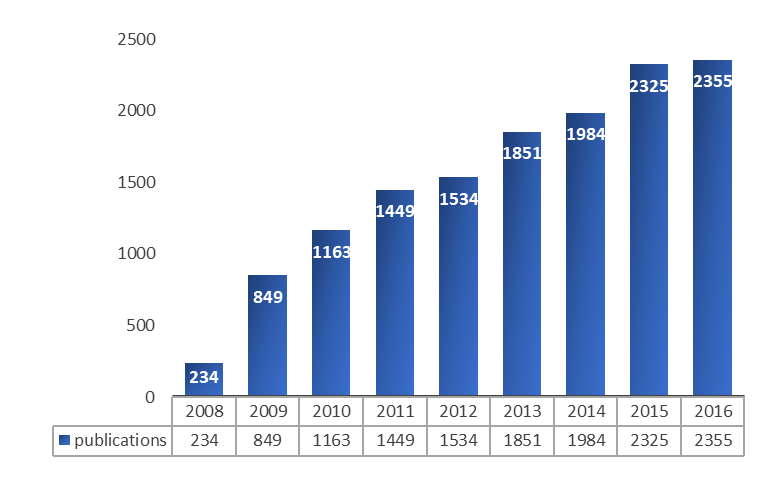
\includegraphics[width=.8\textwidth, height=.6\textheight, keepaspectratio]{chartPubMed}
	\caption[PubMed text mining results]{The number of publications in PubMed using the query word ‘‘\textit{text mining}’’ or ‘‘\textit{literature mining}’’ in the title or abstract over the last years. Search detail: \textit{text mining} [Title/Abstract] or \textit{literature mining} [Title/Abstract].}
	\label{fig:chartPubMed}
\end{figure}


The purpose of Text Mining is to process unstructured (textual) information, extract meaningful numeric indices from the text, and, thus, make the information contained in the text accessible to the various data mining (statistical and machine learning) algorithms. Information can be extracted to derive summaries for the words contained in the documents or to compute summaries for the documents based on the words contained in them. Hence, you can analyze words, clusters of words used in documents, etc., or you could analyze documents and determine similarities between them or how they are related to other variables of interest in the data mining project. In the most general terms, text mining will \enquote*{turn text into numbers} (meaningful indices), which can then be incorporated in other analyses such as predictive data mining projects, the application of unsupervised learning methods (clustering), etc. These methods are described and discussed in great detail in the comprehensive overview work by \citeauthor{manning1999foundations} \citeyear{manning1999foundations}.

Text mining employs many computational technologies, such as machine learning, natural language processing, biostatistics, information technology, and pattern recognition, to find new exciting outcomes hidden in unstructured biomedical text. The goal of text mining is to derive implicit knowledge that hides in unstructured text and present it in an explicit form. This generally has four phases: information retrieval, information extraction, knowledge discovery, and hypothesis generation. Information retrieval systems aim to get desired text on a certain topic; information extraction systems are used to extract predefined types of information such as relation extraction; knowledge discovery systems help us to extract novel knowledge from text; hypothesis generation systems infer unknown biomedical facts based on text. Thus, the general tasks of biomedical text mining include information retrieval, named entity recognition and relation extraction, knowledge discovery and hypothesis generation. \cite{zhu2013biomedical}

To reiterate, text mining can be summarized as a process of \enquote*{numericizing} text. At the simplest level, all words found in the input documents will be indexed and counted in order to compute a table of documents and words, i.e., a matrix of frequencies that enumerates the number of times that each word occurs in each document. This basic process can be further refined to exclude certain common words such as \enquote*{the} and \enquote*{a} (stop word lists) and to combine different grammatical forms of the same words such as \enquote*{traveling}, \enquote*{traveled}, \enquote*{travel}, etc. (This process is known as stemming\footnote{The term stemming refers to the reduction of words to their roots so that, for example, different grammatical forms or declinations of verbs are identified and indexed (counted) as the same word. For example, stemming will ensure that both \enquote*{travel} and \enquote*{traveled} will be recognized by the program as the same word.}). However, once a table of (unique) words (terms) by documents has been derived, all standard statistical and data mining techniques can be applied to derive dimensions or clusters of words or documents, or to identify \enquote*{important} words or terms that best predict another outcome variable of interest.

Once the input documents have been indexed and the initial word frequencies (by document) computed, a number of additional transformations can be performed to summarize and aggregate the information that was extracted.
As described above, the most basic result of the initial indexing of words found in the input documents is a frequency table with simple counts, i.e., the number of times that different words occur in each input document. Usually, we would transform those raw counts to indices that better reflect the (relative) \enquote*{importance} of words and/or their semantic specificity in the context of the set of input documents (see the discussion of inverse document frequencies, above).
A common analytic tool for interpreting the \enquote*{meaning} or \enquote*{semantic space} described by the words that were extracted, and hence by the documents that were analyzed, is to create a mapping of the word and documents into a common space, computed from the word frequencies or transformed word frequencies (e.g., inverse document frequencies).

After significant (e.g., frequent) words have been extracted from a set of input documents, and/or after singular value decomposition has been applied to extract salient semantic dimensions, typically the next and most important step is to use the extracted information in a data mining project.
\begin{itemize}
	\item \textbf{Graphics (visual data mining methods).} Depending on the purpose of the analyses, in some instances the extraction of semantic dimensions alone can be a useful outcome if it clarifies the underlying structure of what is contained in the input documents. For example, a study of new car owners' comments about their vehicles may uncover the salient dimensions in the minds of those drivers when they think about or consider their automobile (or how they \enquote*{feel} about it). For marketing research purposes, that in itself can be a useful and significant result. You can use the graphics (e.g., 2D scatterplots or 3D scatterplots) to help you visualize and identify the semantic space extracted from the input documents.
	\item \textbf{Clustering and factoring.} You can use cluster analysis methods to identify groups of documents (e.g., vehicle owners who described their new cars), to identify groups of similar input texts. This type of analysis also could be extremely useful in the context of market research studies, for example of new car owners. You can also use Factor Analysis and Principal Components and Classification Analysis (to factor analyze words or documents).
	\item \textbf{Predictive data mining.} Another possibility is to use the raw or transformed word counts as predictor variables in predictive data mining projects.
\end{itemize}



In Numeric Natural Language Processing (NLP), we often map words into vectors that contains numeric values so that machine can understand it. Word embedding is a type of mapping that allows words with similar meaning to have similar vectorial representation.



A traditional way of representing words is one-hot vector, which is essentially a vector with only one target element being 1 and the others being 0. The length of the vector is equal to the size of the total unique vocabulary in the corpora. Conventionally, these unique words are encoded in alphabetical order. Namely, you should expect the one-hot vectors for words starting with “a” with target “1” of lower index, while those for words beginning with “z” with target “1” of higher index.


\begin{figure}[ht]
    \centering
    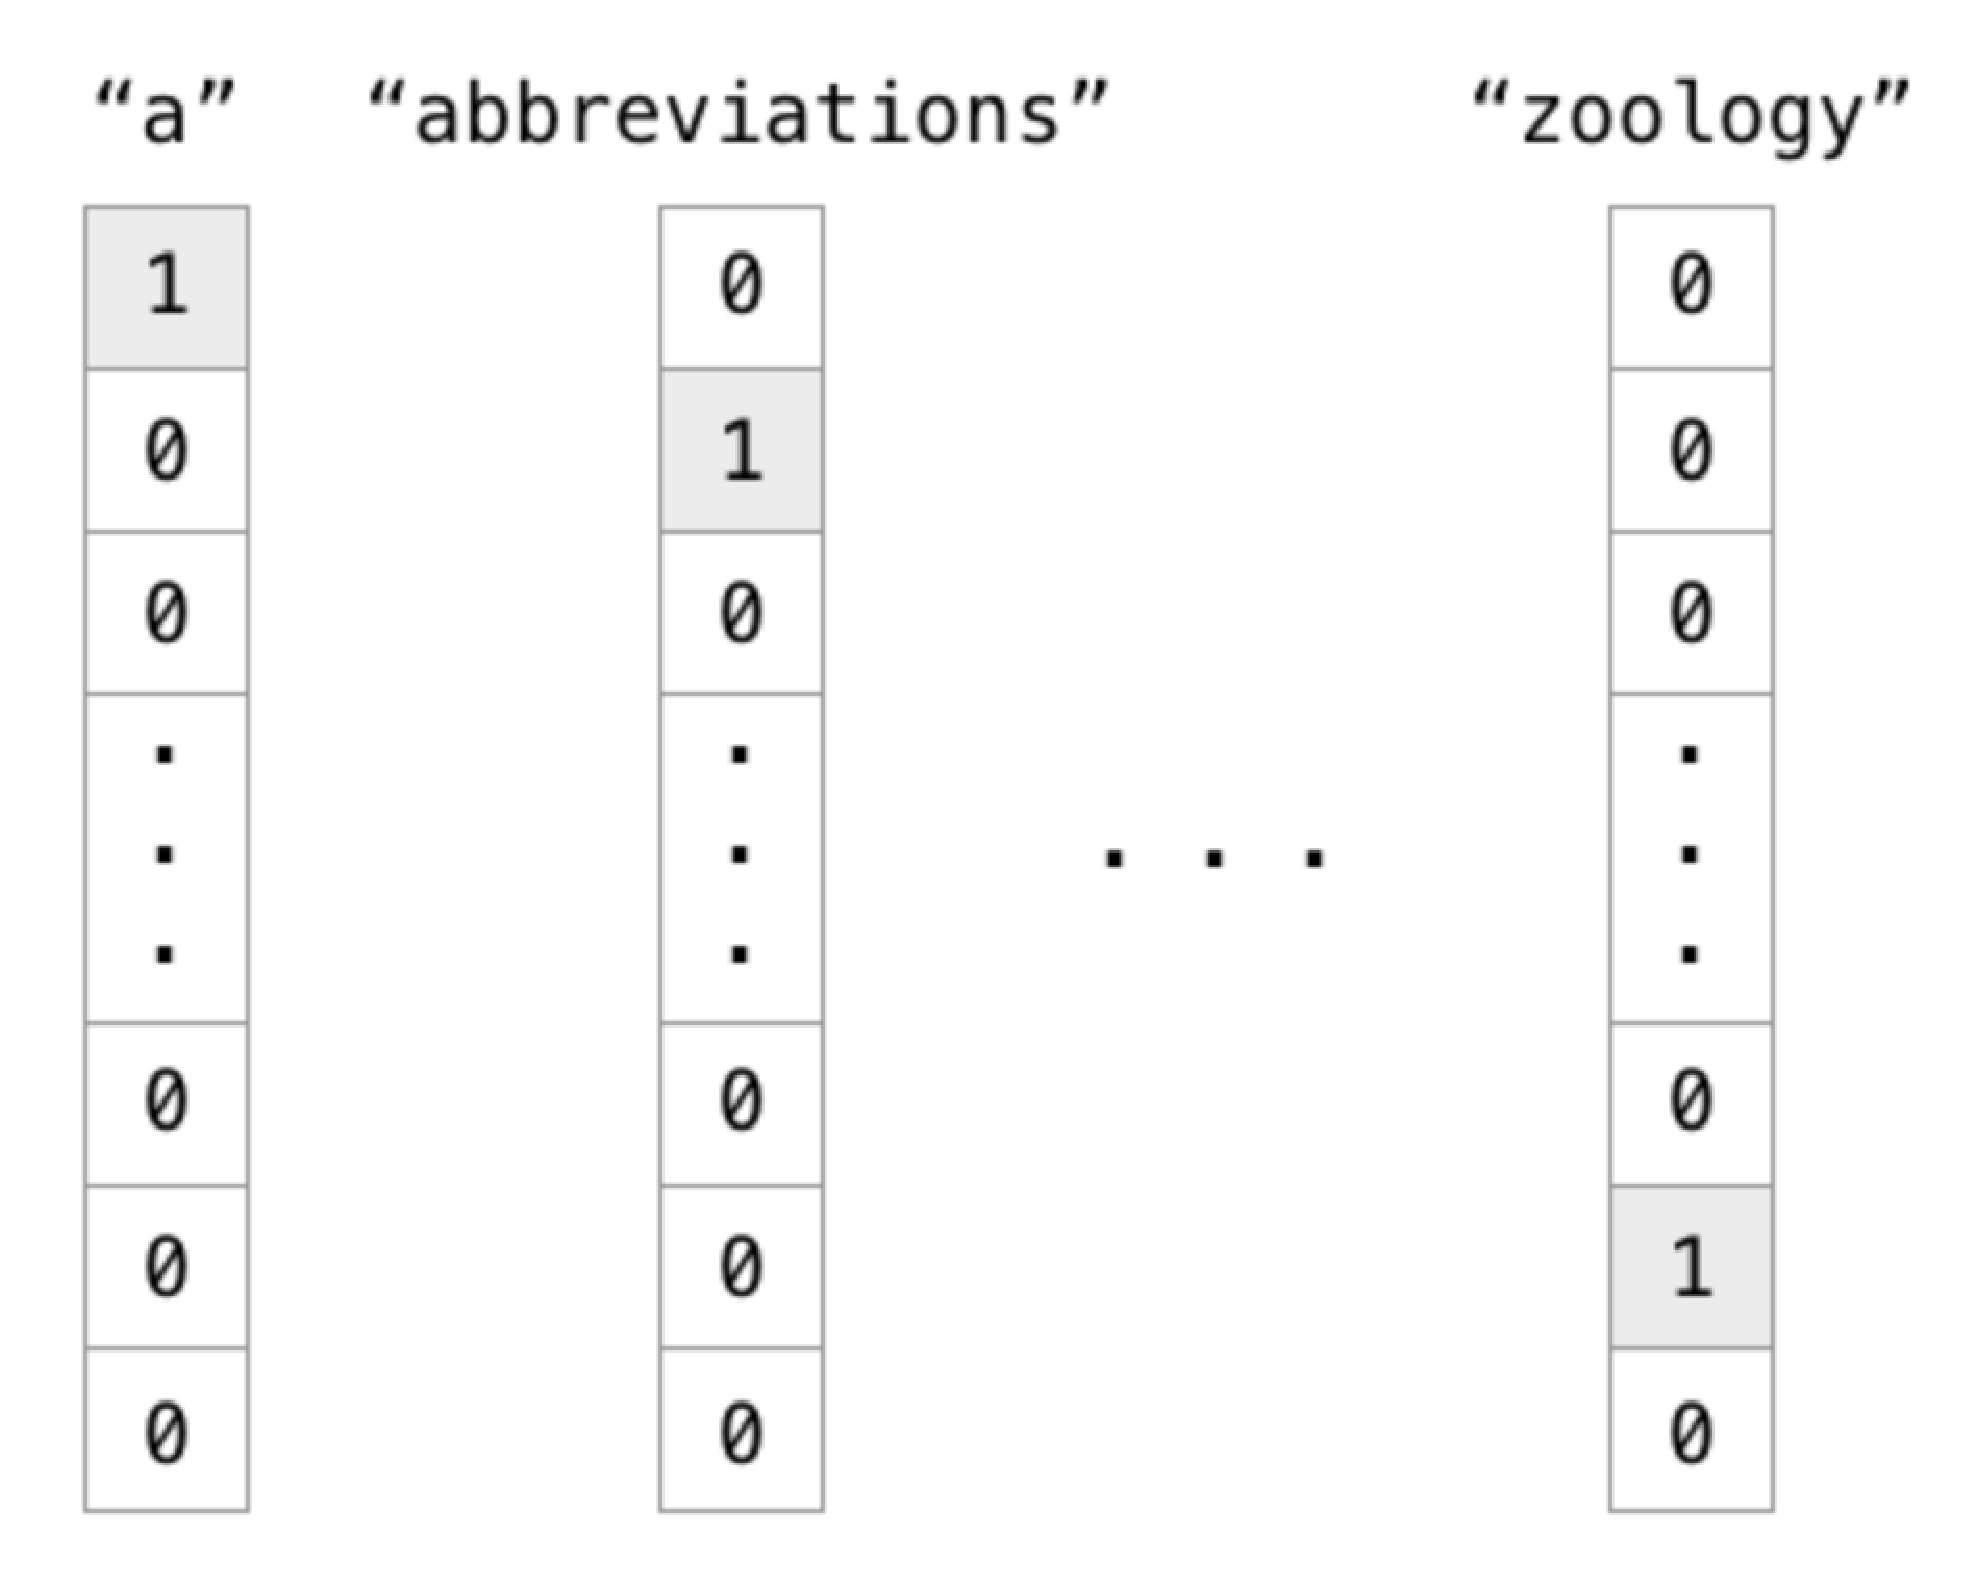
\includegraphics[width=.8\textwidth, height=.6\textheight, keepaspectratio]{1_hot_vector}
    \caption[One Hot vector]{One Hot Vector: A simple and easy way to implement word vectors. 1 Bit set to 1 and all the others to 0. The dimension of the vector depends on the size of the vocabulary in input.}
    \label{fig:1_hot_vector}
\end{figure}

Though this representation of words is simple and easy to implement, there are several issues. First, you cannot infer any relationship between two words given their one-hot representation. For instance, the word “endure” and “tolerate”, although have similar meaning, their targets “1” are far from each other. In addition, sparsity is another issue as there are numerous redundant “0” in the vectors. This means that we are wasting a lot of space.We need a better representation of words to solve these issues.



Word2Vec\footnote{\url{https://code.google.com/archive/p/word2vec/}} is an efficient solution to these problems, which leverages the context of the target words. Essentially, we want to use the surrounding words to represent the target words with a Neural Network whose hidden layer encodes the word representation.

There are two types of Word2Vec, Skip-gram and Continuous Bag of Words (CBOW). I will briefly describe how these two methods work in the following paragraphs.

For skip-gram, the input is the target word, while the outputs are the words surrounding the target words. For instance, in the sentence “I have a cute dog”, the input would be “a”, whereas the output is “I”, “have”, “cute”, and “dog”, assuming the window size is 5. All the input and output data are of the same dimension and one-hot encoded. The network contains 1 hidden layer whose dimension is equal to the embedding size, which is smaller than the input/output vector size. At the end of the output layer, a
softmax activation function is applied so that each element of the output vector describes how likely a specific word will appear in the context.
In mathematics, the softmax function, or normalized exponential function is a generalization of the logistic function that \textit{squashes} a K-dimensional vector z of arbitrary real values to a K-dimensional vector $\delta$(z) of real values, where each entry is in the range (0,1) and all the entries add up to 1. The target is a (K-1)-dimensional space, so one dimension has been lost. \cite{wiki:softmax}

The graph below visualizes the network structure. [Fig \ref{fig:skip_gram}]

\begin{figure}[ht]
	\centering
	\includegraphics[width=.8\textwidth, height=.6\textheight, keepaspectratio]{skip_gram}
	\caption[Skip-gram evaluation]{Skip-gram: The word embedding for the target words can be obtained by extracting hidden layers after feeding the one-hot representation of that word into the network.}
	\label{fig:skip_gram}
\end{figure}

With skip-gram, the representation dimension decreases from the vocabulary size (V) to the length of the hidden layer (N). Furthermore, the vectors are more “meaningful” in terms of describing the relationship between words. The vectors obtained by subtracting two related words sometimes express a meaningful concept such as gender or verb tense, as shown in the following figure (dimensionality reduced). [Fig \ref{fig:skip_gram_2}]

\begin{figure}[ht]
	\centering
	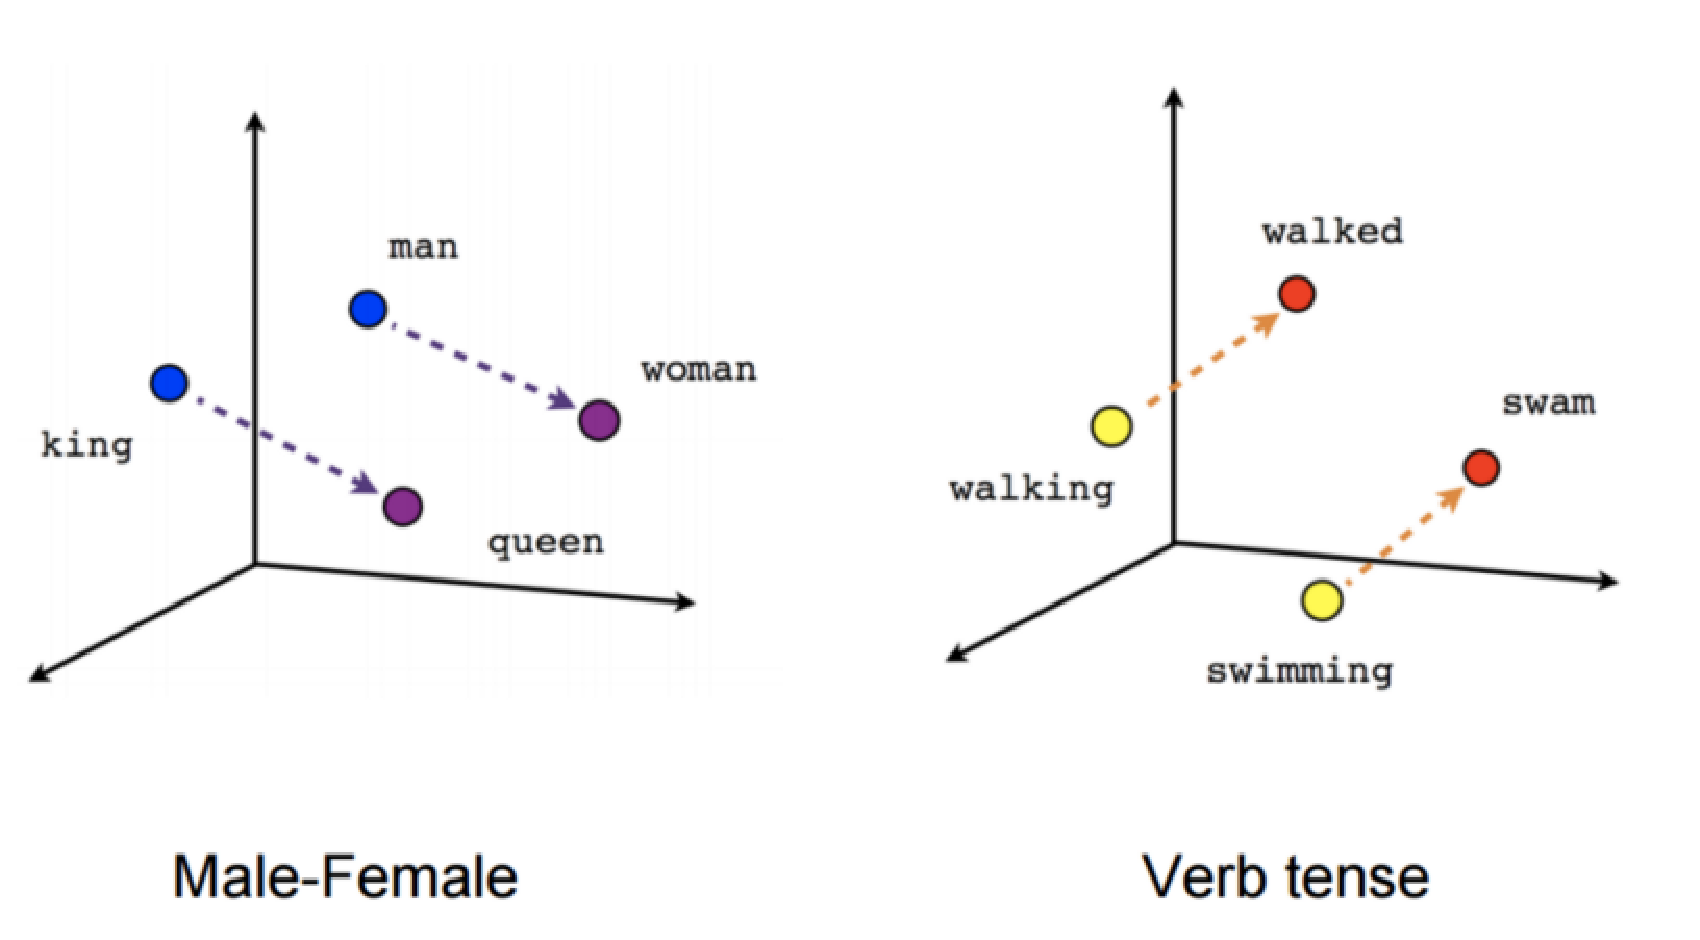
\includegraphics[width=.9\textwidth, height=.9\textheight, keepaspectratio]{skip_gram_2}
	\caption[Skip-gram relationship between words]{Skip-gram: the vectors are more "meaningful" in terms of describing the relationship between words.}
	\label{fig:skip_gram_2}
\end{figure}



Continuous Bag of Words (CBOW)\footnote{\url{https://iksinc.online/tag/continuous-bag-of-words-cbow/}} is very similar to skip-gram, except that it swaps the input and output. The idea is that given a context, we want to know which word is most likely to appear in it.

\begin{figure}[ht]
	\centering
	\includegraphics[width=0.8\textwidth, height=0.6\textheight, keepaspectratio]{cbow}
	\caption[CBOW and Skip-gram]{The main difference between CBOW and Skip-gram is that CBOW swaps the input and output.}
	\label{fig:cbow}
\end{figure}


The biggest difference between Skip-gram and CBOW is that the way the word vectors are generated. For CBOW, all the examples with the target word as target are fed into the networks, and taking the average of the extracted hidden layer. For example, assume we only have two sentences, “He is a nice guy” and “She is a wise queen”. To compute the word representation for the word “a”, we need to feed in these two examples, “He is nice guy”, and “She is wise queen” into the Neural Network and take the average of the value in the hidden layer. Skip-gram only feed in the one and only one target word one-hot vector as input.

Figure \ref{fig:cbow} shows a 3D representation of word vectors, after a applying a nonlinear dimensionality reduction function like (t-SNE)\footnote{t-distributed Stochastic Neighbor Embedding}\cite{maaten2008visualizing}. The key to understand here is that having the vectors in 2 or 3 dimensions we can then move in some direction and find terms given by the contest. If we move through the male-female direction from the word vector representing the word \textit{man}, we are likely to find the word \textit{woman}. Likewise we are going to find the word \textit{queen} if we start from the word vector representing the word \textit{queen}.

It is claimed that Skip-gram tends to do better in rare words. Nevertheless, the performance of Skip-gram and CBOW are generally similar.



FastText is an extension to Word2Vec proposed by Facebook in 2016. Instead of feeding individual words into the Neural Network, FastText breaks words into several n-grams (sub-words). For instance, the tri-grams for the word apple is app, ppl, and ple (ignoring the starting and ending of boundaries of words). The word embedding vector for apple will be the sum of all these n-grams. After training the Neural Network, we will have word embeddings for all the n-grams given the training dataset. Rare words can now be properly represented since it is highly likely that some of their n-grams also appears in other words.\cite{word2vecFastText}


Due to the success of word embeddings in a variety of NLP applications, some existing studies evaluate word embeddings in representing word semantics quantitatively. Most of them focus on evaluating the word embeddings generated by different approaches. \citeauthor{baroni2014don} \cite{baroni2014don} presented the first systematic evaluation of word embeddings generated by four models, i.e., DISSECT, CBOW using word2vec, Distributional Memory model, and Collobert and Weston model using a corpus of 2.8 billion tokens in the general English domain. They tested these models on fourteen benchmark datasets in five categories, including semantic relatedness, synonym detection, concept categorization, selectional preferences, and analogy. They found that the word2vec model, CBOW, performed the best for almost all the tasks. \citeauthor{schnabel2015evaluation} \cite{schnabel2015evaluation} trained the CBOW model of word2vec, C\&W embeddings \cite{collobert2011natural} , Hellinger PCA \cite{lebret2013word}, GloVe \cite{pennington2014glove}, TSCCA \cite{dhillon2012two}, and Sparse Random Projections \cite{li2006very} on a 2008 GloVe dump, and tested on the same fourteen datasets. They found that the CBOW outperformed other embeddings on 10 datasets. They also conducted an extrinsic evaluation by using the embeddings as input features to two downstream tasks, namely noun phrase chunking and sentiment classification. They found the results of CBOW were also among the best.
\citeauthor{ghannay2016word} \cite{ghannay2016word} conducted a similar intrinsic evaluation, they additionally evaluated the skip-gram models of word2vec, CSLM word embeddings \cite{schwenk2013cslm}, dependency-based word embeddings, and combined word embeddings on four NLP tasks, including Part-Of-Speech tagging, chunking, named entity recognition, mention detection, and two linguistic tasks. They trained these word embeddings on the Gigaword corpus composed of 4 billion words and found that the dependency-based word embeddings gave the best performance on the NLP tasks and that the combination of embeddings yielded significant improvement. However, few of these studies evaluated word embeddings for tasks in the biomedical domain.
As most of the aforementioned studies evaluate word embeddings in the general (i.e., non-biomedical) NLP domain, only one recent study by \citeauthor{pakhomov2016corpus} \cite{pakhomov2016corpus} evaluates word embeddings in the biomedical domain, to the best of our knowledge. They trained the CBOW model on two biomedical corpora, namely clinical notes and biomedical publications, and one general English corpora, namely GloVe. The word embeddings were evaluated on subsets of UMNSRS dataset, which consisted of pairs of medical terms with the similarity of each pair assessed by medical experts, and on a document retrieval task and a word sense disambiguation task. They found that the semantics captured by the embeddings computed from biomedical publications were on par with that from clinical notes.



There is a rich body of work on learning general-purpose word embeddings. So far, there are only very few studies focusing on learning domain-specific word embeddings. For example, \citeauthor{ghosh2016designing} \citeyear{ghosh2016designing} \cite{ghosh2016designing} uses information from a disease lexicon to generate disease-specific word embeddings. The main objective is to bring in-domain words close to each other in the embedding space while pushing out-domain words away from in-domain words. \citeauthor{ghosh2016designing} \citeyear{ghosh2016designing} \cite{ghosh2016designing} only concerns whether a word is in-domain or not.
Another example is \citeauthor{domainSpecificWordEmbedding} \citeyear{domainSpecificWordEmbedding} \cite{domainSpecificWordEmbedding}, describes a novel method to train domain-specific word embeddings from sparse texts. First, it proposes a general framework to encode diverse types of domain knowledge as text annotations; then, it develops a novel Word Annotation Embedding (WAE) algorithm to incorporate diverse types of text annotations in word embedding. Evaluating the method on two text corpora resulted in demonstrating the effectiveness of the method in learning domain-specific word embeddings.



The existing studies of automating ICD-9-CM code assignment can be classified into two groups. Through examining how professional coders assigning ICD-9-CM codes, the first one used rule-based approaches. \citeauthor{goldstein2007three} \citeyear{goldstein2007three} \cite{goldstein2007three} developed a rulebased system considering factors such as uncertainty, negation, synonymy, and lexical elements.
\citeauthor{farkas2008automatic} \citeyear{farkas2008automatic} \cite{farkas2008automatic} used Decision Tree (DT) and Maximum Entropy (ME) to automatically generate a rule-based coding system. \citeauthor{crammer2007automatic} \citeyear{crammer2007automatic} \cite{crammer2007automatic} composed a hybrid system consisting of a machine learning system with natural language features, a rule-based system based on the overlap between the reports and code descriptions, and an automatic policy system. Their results showed better performance than each single system. The second group employed supervised machine learning methods for the assignment task, and their performance has been being equivalent or even better than those rule-based systems that need experts manually crafting knowledge. \citeauthor{aronson2007indexing} \citeyear{aronson2007indexing} \cite{aronson2007indexing} used a stacked model to combine the results of four modules: Support Vector Machine (SVM), K-Nearest Neighbors (KNN), Pattern Matching (PM) and a hybrid Medical Text Indexer (MTI) system. \citeauthor{patrick2007developing} \citeyear{patrick2007developing} \cite{patrick2007developing} used ME and SVM classifiers, enhanced by a feature engineering module that explores the best combination of several types of features. \citeauthor{zhang2008hierarchical} \citeyear{zhang2008hierarchical} \cite{zhang2008hierarchical} proposed a hierarchical text categorization method utilizing the ICD-9-CM codes structure.
Along with the introduction of supervised methods, many past studies indicated that data imbalance problem can severely affect the classifier’s performance. For example, \citeauthor{kavuluru2015empirical} \citeyear{kavuluru2015empirical} \cite{kavuluru2015empirical} found that 874 of 1,231 ICD-9-CM codes in UKLarge dataset have less than 350 supporting data, whereas only 92 codes have more than 1,430 supporting data. The former group has macro F1 value of 51.3\%, but the latter group only has 16.1\%. To resolve data imbalance problem, they used optimal training set (OTS) selection approach to sample negative instance subset that provides best performance on validation set. However, OTS did not work on UKLarge dataset because several codes have so few training examples that even carefully selecting negative instances could not help. When \citeauthor{koopman2015automatic} \citeyear{koopman2015automatic} \cite{koopman2015automatic} found that 85\% of the whole death certificate dataset is associated with only top 20 common cancers, whereas the other 65 rarer cancers only have the rest 15\% of the dataset, they tried to construct the balanced training set by randomly sampling a static number of negative examples for each class. Their results reflected the benefits of having more training data in improving the classifiers’ performance. 
Since result of original model learned with imbalanced data is not provided, we cannot know the actual improvement. In addition, to deal with codes that only appear once in the dataset, \citeauthor{patrick2007developing} \citeyear{patrick2007developing} \cite{patrick2007developing} used a rule-based module to supplement ME and SVM classifiers.
For the recent studies, \citeauthor{zhao2017automatic} \citeyear{zhao2017automatic} \cite{zhao2017automatic} proposed an automatic feature extraction method, capturing semantic relational tuples. They proved the semantic relational tuple is able to capture information at semantic level and it contribute to ICD-9-CM classification task in two aspects, negation identification and feature generation. Another recent study to solve training data shortage problem, \citeauthor{zhang2017enhancing} \citeyear{zhang2017enhancing} \cite{zhang2017enhancing} proposed to strategically draw data from PubMed to enrich the training data when there is such need. The evaluation results indicate that their method can significantly improve the code assignment classifiers’ performance at the macro-averaging level. 